\documentclass[border=3pt]{standalone}
\usepackage{fontspec,amsmath,amssymb,newtxmath,bm,tikz}
\setmainfont{TeX Gyre Termes}
\usetikzlibrary{arrows.meta,positioning,calc}
\newcommand{\E}{\mathbb E}
\newcommand{\TV}{\operatorname{TV}}
\begin{document}
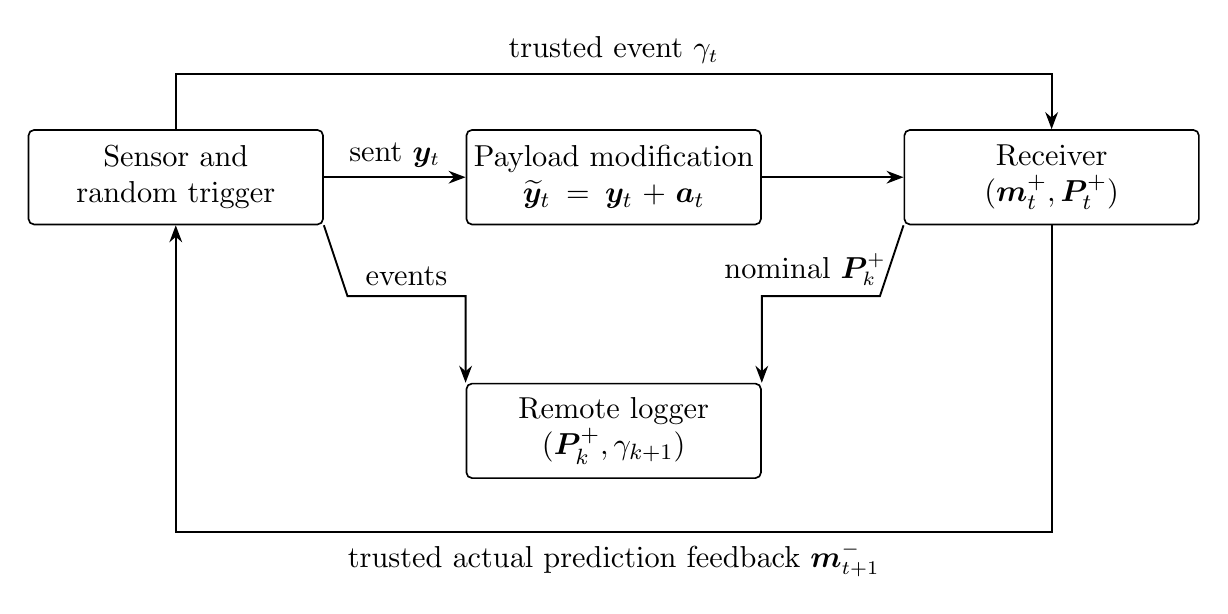
\begin{tikzpicture}[>=Stealth,font=\fontsize{11}{13}\selectfont,
 box/.style={draw,line width=.6pt,rounded corners=2pt,align=center,minimum height=12mm,text width=36mm,inner xsep=2pt},
 edge/.style={->,line width=.7pt},
 edge label/.style={font=\fontsize{10.5}{12.5}\selectfont}]
\node[box] (sensor) {Sensor and\\random trigger};
\node[box,right=18mm of sensor] (attack) {Payload modification\\$\widetilde {\bm{y}}_t={\bm{y}}_t+{\bm{a}}_t$};
\node[box,right=18mm of attack] (receiver) {Receiver\\$({\bm{m}}_t^+,{\bm{P}}_t^+)$};
\node[box,below=20mm of attack] (logger) {Remote logger\\$({\bm{P}}_k^+,\gamma_{k+1})$};
\draw[edge] (sensor) -- node[above,edge label]{sent ${\bm{y}}_t$} (attack);
\draw[edge] (attack) -- (receiver);
\draw[edge] (sensor.north) -- ++(0,7mm) -| node[pos=.25,above,edge label]{trusted event $\gamma_t$} (receiver.north);
\draw[edge] (receiver.south) -- ++(0,-39mm) -| node[pos=.25,below,edge label]{trusted actual prediction feedback ${\bm{m}}_{t+1}^-$} (sensor.south);
\draw[edge] (sensor.south east) -- ++(3mm,-9mm) -| node[pos=.25,above,edge label]{events} (logger.north west);
\draw[edge] (receiver.south west) -- ++(-3mm,-9mm) coordinate (covturn)
 -- node[midway,above,edge label,xshift=-2mm]{nominal ${\bm{P}}_k^+$} (logger.north east |- covturn) -- (logger.north east);
\end{tikzpicture}
\end{document}
